\section{Aufbau und Durchführung}
\label{sec:AufbauUndDurchführung}
\subsection{Aufbau}
\label{sec:Aufbau}
Der grundlegende Aufbau ist in der Abbildung \autoref{fig:Versuchsaufbau} zu erkennen.
Dieser besteht aus einem Justierlaser, einer Blende, zwei Resonatorspiegeln und einem Laserrohr. In dem Laserrohr befinden sich 
Die Komponenten sind alle auf einer optischen Bank
Die  sind auf einer optischen Bank 
\begin{figure}
    \centering
    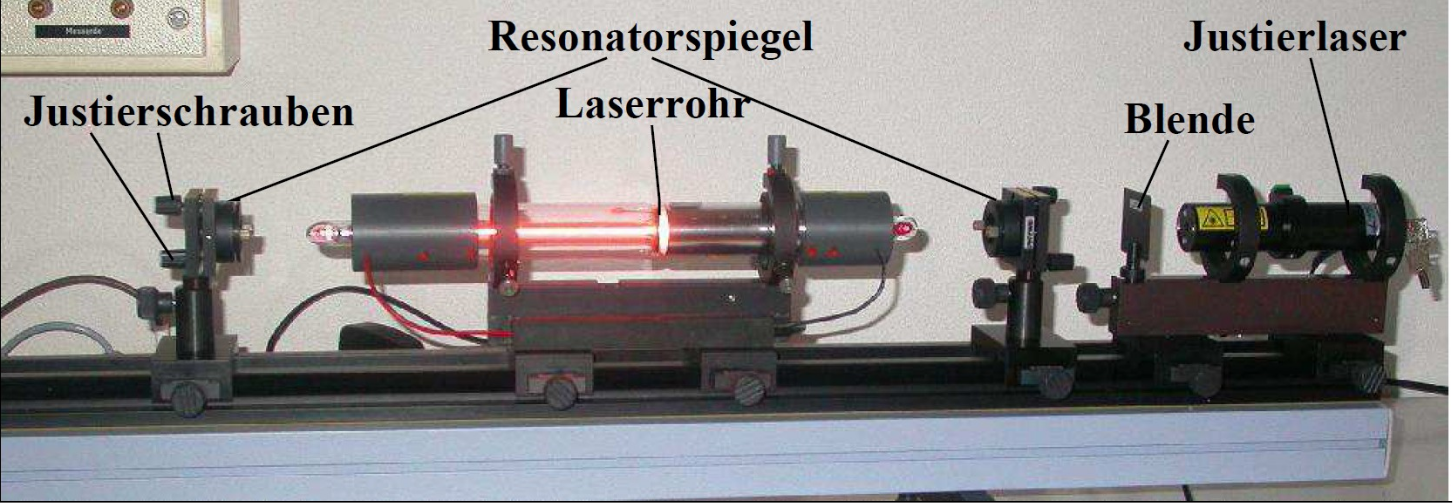
\includegraphics[width=0.75\textwidth]{Bilder/Aufbau.png}
    \caption{Der schematische Aufbau für den He-Ne Laser. \cite{anleitungV61}}
    \label{fig:Versuchsaufbau}
  \end{figure}

\subsection{Durchführung}
\label{sec:Durchführung}